% !TEX root = ../main.tex

\section{Supply Rail Ripple}
\label{sec:results-supply}

\scaffold{
  \textbf{Paragraph 1, setup.} The ripple of the input (VEXT, TP15) and the three rails (TP12--TP14) was measured AC-coupled at 1X in four operating states: without microcontroller, idle or detecting, following a pedal, and following with WiFi active. Per rail and state, the RMS value averaged over 70 to 1000 acquisitions at \qty{10}{\milli\second}/div (high-resolution mode) is reported; captures at \qty{1}{\micro\second}/div reached the oscilloscope's own noise at every rail and are not shown. The noise floor of the oscilloscope, \qty{0.34}{\milli\volt} RMS, was taken under the same settings. The values were read from the oscilloscope's statistics by a script and checked by hand.
}

\scaffold{
  \textbf{Paragraph 2, the limit.} Derive the ripple that would just disturb a stable 7-bit value, drawn in \cref{fig:supply-ripple}: one MIDI step of the \qty{2.5}{\volt} reference is $\qty{2.5}{\volt}/128 = \qty{19.5}{\milli\volt}$, and requiring $\pm 3\sigma$ of Gaussian noise to fit into one step gives $\qty{19.5}{\milli\volt}/6 = \qty{3.26}{\milli\volt}$ RMS. Use the same step as \cref{sec:results-position} (1/127 of the span); the plot divides by 128, a difference below \qty{1}{\percent} that should still be made consistent in \code{create\_plots.py}. One sentence on why this is conservative: the reading is ratiometric, so ripple common to the pull rail and the reference cancels further.
}

\begin{figure}[htbp]
  \centering
  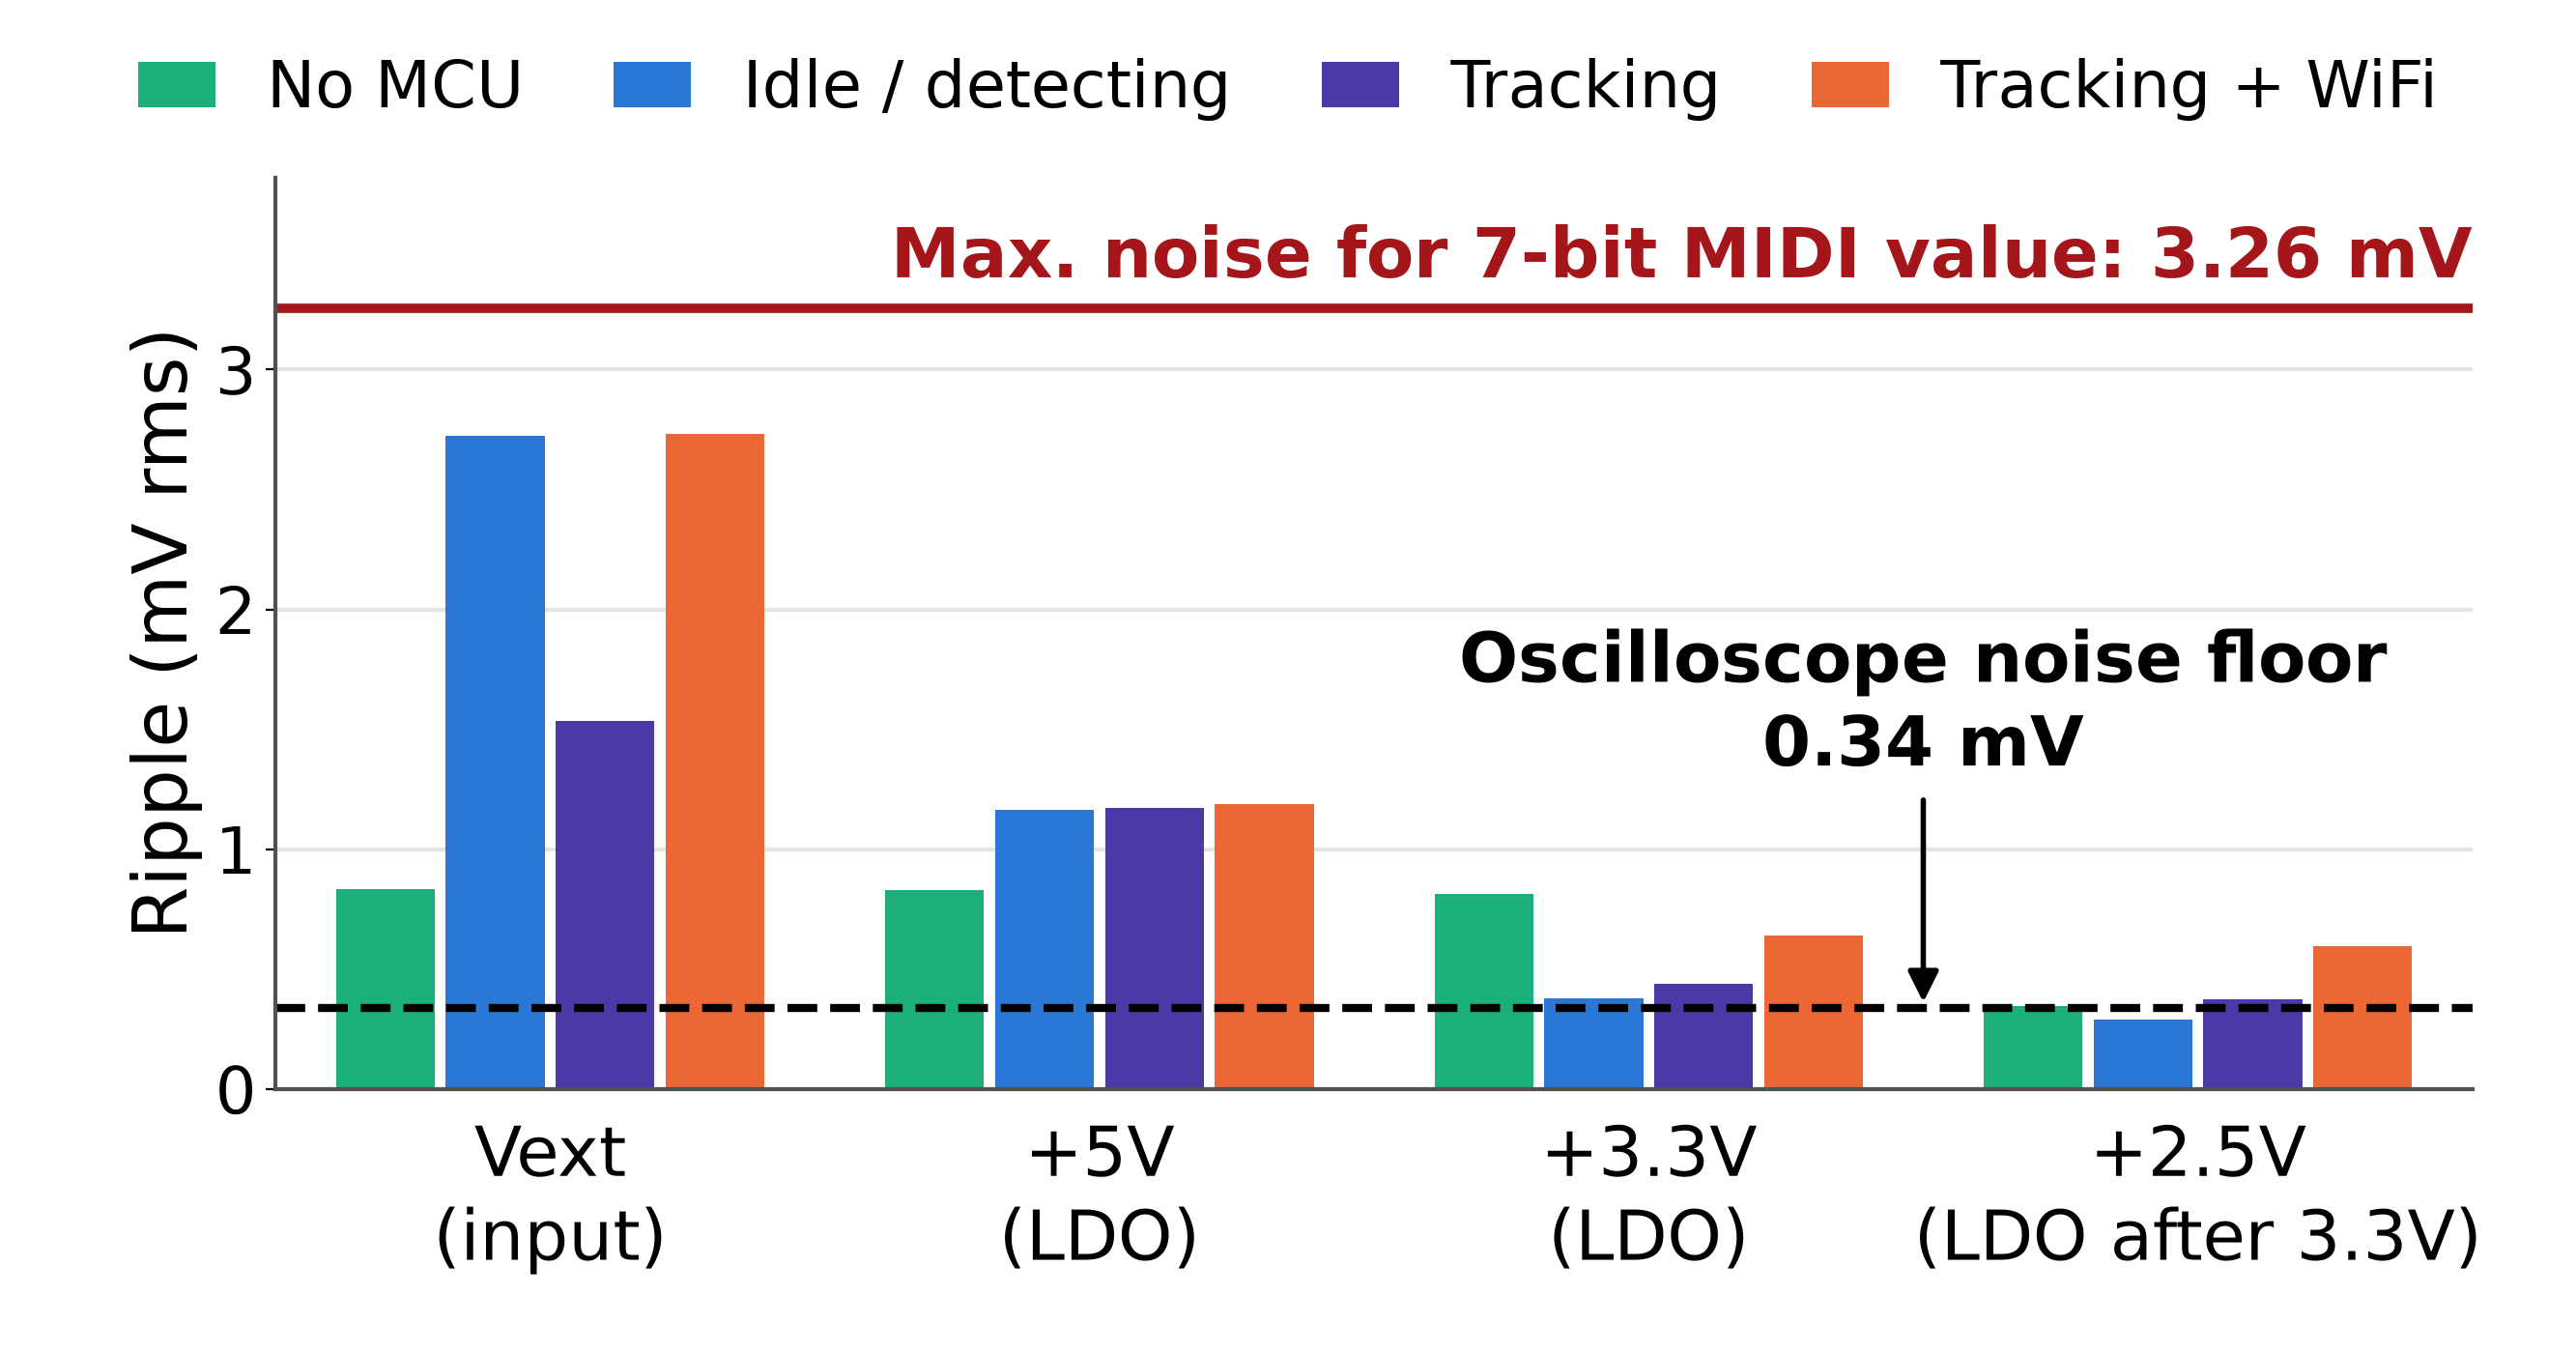
\includegraphics[width=\linewidth]{05-results/figures/supply-rail-ripple}
  \titledcaption{Supply Rail Ripple}{\scaffoldinline{State the conditions (AC coupling, 1X probe, \qty{10}{\milli\second}/div, RMS average), name the four operating states, the oscilloscope noise floor and the limit for a stable 7-bit value. Rails are ordered along the regulator chain. Source: \code{measurements/create\_plots.py}, data \code{measurements/supply\_rail\_measurement.xlsx}.}}
  \label{fig:supply-ripple}
\end{figure}

\scaffold{
  \textbf{Paragraph 3, what the data shows.} The input ripple rises from \qty{0.83}{\milli\volt} without microcontroller to about \qty{2.7}{\milli\volt} RMS once the microcontroller runs; read the exact values per state from the plot, which shows the state \enquote{idle / detecting} as high as \enquote{tracking + WiFi} and \enquote{tracking} lower, and explain or flag this. Every regulator stage lowers it, and the \qty{3.3}{\volt} and \qty{2.5}{\volt} rails stay between 0.3 and \qty{0.6}{\milli\volt}, at or just above the noise floor, so their exact values are not meaningful. WiFi is the only state that visibly raises them. The \qty{5}{\volt} rail shows about \qty{1.2}{\milli\volt} RMS but about \qty{16}{\milli\volt} peak-to-peak once the microcontroller runs, i.e. short spikes rather than broadband noise. Every rail stays below the \qty{3.26}{\milli\volt} limit; the \qty{2.5}{\volt} rail by a factor of about five even with WiFi.
}

\openquestion{Supply data quality}{
  Three readings without microcontroller (VEXT, \qty{5}{\volt}, \qty{3.3}{\volt}) were taken without resetting the oscilloscope statistics between rails, which makes the \qty{3.3}{\volt} rail look worse without the microcontroller than with it. Decide whether to remeasure, mark or drop them. Confirm that the noise floor capture (image~2) was taken with the probe tip on the ground pad, and give the cause of the spikes on the \qty{5}{\volt} rail if known (suspected: the switching regulator of the Pico module).
}
